
\documentclass{ppgeesa}

%%%%%%%%%%%%%%%%%%%%%%%%%%%%%%%%%%%%%%%%%%%%%%%%%%%%%%%%%%%%%%%%%%%%%%%%%%%%%%%%%%%%%%%%%%%%%%%%%%%%%%%%%%%%%%%%%

\usepackage[latin1]{inputenc}
\usepackage{graphicx}
\usepackage{hyperref}
\usepackage{tikz}
\usepackage{amsmath}
\usepackage{listings}

\lstset{stepnumber=2, frame=single,tabsize=2, breaklines=true, basicstyle=\footnotesize}

\hypersetup{
	colorlinks,
	debug=true,
	linkcolor=black,  %%% cor do tableofcontents, \ref, \footnote, etc
	citecolor=red,  %%% cor do \cite
	urlcolor=blue,   %%% cor do \url e \href
	bookmarksopen=true,
	pdftitle={Controle Robusto},
	pdfauthor={Tassiano Neuhaus},
	pdfsubject={Sistemas de controle multivari�veis},
	pdfkeywords={Controle Robusto}
	%pdfpagemode=FullScreen
}

%%%%%%%%%%%%%%%%%%%%%%%%%%%%%%%%%%%%%%%%%%%%%%%%%%%%%%%%%%%%%%%%%%%%%%%%%%%%%%%%%%%%%%%%%%%%%%%%%%%%%%%%%%%%%%%%%


\begin{document}

\title{Controle Robusto e Caracteriza��o de incertezas}

\author{Tassiano Neuhaus\\
{\small Universidade Federal do Rio Grande do Sul - Departamento de Engenharia El�trica\\Av. Osvaldo Aranha, 103 - Bairro Bom Fim CEP: 90035-190 - Porto Alegre - RS - Brazil}\\
}%\thanks{Tassiano Neuhaus, tassianors@gmail.com, tel +55-51-91760154}}

\maketitle
\thispagestyle{empty}\pagestyle{empty}

\begin{abstract}
Neste trabalho ser� apresentado a caracteriza��o de um sistema sujeito a incertezas. A caracteriza��o
ser� baseada nos seguintes tipos: Polit�picas, limitadas em norma, diagonal e elemento por elemento.

Para cada uma das incertezas caracterizadas ser� projetada uma realimenta��o de estados para minimizar
a norma {\it{H2}} em malha fechada. O mesmo ser� feito para minimizar a norma {\it{$H_{\infty}$}}
\end{abstract}

\begin{IEEEkeywords}
Controle Robusto, Incertezas polit�picas, limitadas em norma e diagonais.
\end{IEEEkeywords}

%===============================================================================
\section{Introdu��o}

Neste trabalho ser� apresentado o projeto de controladores denominados Robustos. Para 
tanto ser� apresentado o conceito de um controlador Robusto. A fim de modelar um
sistema sujeito a incertezas ser� apresentado alguns m�todos para que sua modelagem
matem�tica seja poss�vel. 

Para tornar o estudo mais claro ser� utilizado um sistema f�sico onde estar� sujeito a
perturba��es e/ou incertezas. Sobre este sistema ser� feito a modelagem seguindo cada um
dos processos e com estes modelos ser� efetuado uma simula��o. 

Esta simula��o ser� baseada no projeto de uma realimenta��o de estados com o intuito de
satisfazer a minimiza��o da norma $H2$ e $H_{\infty}$.

O sistema utilizado � apresentado no sistema de equa��es de estado descrito em (\ref{eq:intro_sis}).

\begin{equation}
\begin{matrix}
A=\begin{bmatrix}
0 & 1\\ 
-ba &a+b 
\end{bmatrix} &
B=\begin{bmatrix}
0\\ 
k
\end{bmatrix} 
\end{matrix}
\label{eq:intro_sis}
\end{equation}

Este sistema possui a fun��o de transfer�ncia apresentado em (\ref{eq:intro_transf}).

\begin{equation}
G(s)=\frac{k}{(s-a)(s-b)}
\label{eq:intro_transf}
\end{equation}

Os par�metros $a, b, k$ est�o sujeitos as varia��es apresentadas em (\ref{eq:intro_limit}).

\begin{equation}
\begin{matrix}
b= & -0.012725 & \\ 
k= & [k_1 \; k_2] =& [-0.4649.10^{-4} \; -0.7449.10^{-4}]\\ 
a= & [a_1 \; a_2] =& [-0.25 \; -2]
\end{matrix}
\label{eq:intro_limit}
\end{equation}


\section{Caracteriza��o}
\label{sec:caracterization}

%===============================================================================
\subsection{Polit�pica}
\label{sec:carac_politopica}

%===============================================================================
\subsection{Limitada em norma} 
\label{sec:carac_limit_norma}

%===============================================================================
\subsection{Diagonais}
\label{sec:carac_diagonais}

%===============================================================================
\subsection{Elemento a elemento}
\label{sec:carac_elemento}



\section{Controle Robusto}
\label{sec:robust}
%===============================================================================

Nas se��es seguintes ser� apresentado a modelagem para os tipos de incertezas.
Utilizando o sistema descrito em (\ref{eq:intro_sis}) e os limites das incertezas
descritos em (\ref{eq:intro_limit}), ser� apresentada a modelagem baseado em cada
um dos tipos apresentados a seguir.

%===============================================================================
\subsubsection{Estabilidade quadr�tica}
\label{sec:robust_quadratic}

A ideia fundamental da estabiliza��o quadr�tica de um sistema incerto aut�nomo 
por realimenta��o linear est�tica de estados � encontrar uma lei de controle tal
que a fun��o quadr�tica definida positiva:

\begin{equation}
V(x)=x'Px; \; com P>0
\nonumber
\end{equation}

Possua sua derivada definida negativa ao longo da trajet�ria do sistema em malha fechada:

\begin{equation}
\begin{matrix}
\dot{V}(x)=x'\{(A-BK)'P+P(A-BK)\}x < 0\\ 
\forall A \in \mathbf{A}, \forall B \in \mathbf{B}
\end{matrix}
\nonumber
\end{equation}

Desta forma o que busca-se � uma matriz $P$ que satisfa�a n�o apenas uma equa��o mas
um grupo de equa��es para estabilizar o sistema de forma Robusta.

Para um sistema sem incertezas tem-se que a solu��o do problema � como abaixo:

\begin{equation}
P=W^{-1}; K=RW^{-1}
\nonumber
\end{equation}

Para o sistema abaixo com $R\equiv KP^{-1}$.

\begin{equation}
WA_0'+A_0W -B_0R-R'B_0 < 0
\nonumber
\end{equation}

%===============================================================================
\subsection{Polit�pica}
\label{sec:robust_politopica}

Para o caso de incertezas do tipo polit�pico uma condi��o necess�ria e suficiente para a
estabilidade quadr�tica do sistema incerto aut�nomo em malha fechada � que todos os v�rtices
do poliedro que constituem o conjunto de modelos possuam a mesma matriz $P$ sim�trica
definida positiva como matriz de Lyapunov.

\begin{equation}
WA_i'+A_iW-B_jR-R'B_j'< 0
\label{eq:robust_politopico}
\end{equation}

Para $\forall i=1,...,na, \forall j=1,...,nb$.

O sistema utilizado neste trabalho (\ref{eq:intro_sis}) � caracterizado utilizando a
forma polit�pica como em (\ref{eq:carac_sis_politopico}).

\begin{equation}
\begin{matrix}
A_1=\begin{bmatrix}
0 & 1\\ 
-ba_1 &a_1+b 
\end{bmatrix} \; A_2=\begin{bmatrix}
0 & 1 \\ 
-ba_2 & a_2+b 
\end{bmatrix}
\\ \; & \; \\
B_1=\begin{bmatrix}
0\\ 
k_1
\end{bmatrix}B_2=\begin{bmatrix}
0\\ 
k_2
\end{bmatrix}
\end{matrix}
\label{eq:carac_sis_politopico}
\end{equation}

A partir de (\ref{eq:robust_politopico}) tem-se o conjunto de inequa��es lineares apresentado
em (\ref{eq:robust_politopico_equations}).

\begin{equation}
\begin{matrix}
WA_1'+A_1W-B_1R-R'B_1'<0\\ 
WA_1'+A_1W-B_2R-R'B_2'<0\\ 
WA_2'+A_2W-B_1R-R'B_1'<0\\ 
WA_2'+A_2W-B_2R-R'B_2'<0
\end{matrix}
\label{eq:robust_politopico_equations}
\end{equation}

%===============================================================================
\subsection{Limitada em norma}
\label{sec:carac_limit_norma}

Considerando o sistema apresentado em (\ref{eq:robust_sis_incert}) com $\omega(t) \equiv 0$.

\begin{equation}
\left\{\begin{matrix}
\dot{x}(t)=A_0x(t)+B_0u(t)B_{\omega}\omega(t)+Dp(t)
\\ 
q(t)=E_Ax(t)+E_Bu(t)+Fp(t)
\\ 
z(t)=Gx(t)+Hu(t)
\\
p(t)=\Delta(t)q(t); \; \left \| \Delta(t) \right \| \leq 1
\end{matrix}\right.
\label{eq:robust_sis_incert}
\end{equation}

Para este sistema temos que a derivada da fun��o $V(x)=x'Px$ seja definida positiva:

\begin{equation}
x'-(A_0-B_0 K)'P-P(A_0-B_0 K)x-x'PDp-p'D'Px < 0
\nonumber
\end{equation}

Para todo $x \neq 0$ tal que $p'p \leq q'q$ implica de maneira equivalente:

\begin{equation}
p'p \leq ((E_A-E_B K)x)'(E_A-E_B K)x
\nonumber
\end{equation}

Tem-se ent�o que o sistema apresentado em (\ref{eq:robust_limit_norma}) � uma condi��o
necess�ria e suficiente para a estabilidade quadr�tica do sistema com incertezas limitadas
em norma e tamb�m � convexa, portanto pode ser resolvida com algoritmos de resolu��o de LMI.

\begin{equation}
\begin{bmatrix}
-A_0+B_0R-WA_0'+R'B_0'-DD' & -(WE_A+RE_B')\\ 
-(WE_A'+R'E_B')' & I
\end{bmatrix}>0
\label{eq:robust_limit_norma}
\end{equation}

Desta forma para o sistema (\ref{eq:intro_sis}) temos que a modelagem para incertezas limitadas
em norma � a apresentada em (\ref{eq:robust_sis_limit}).

\begin{equation}
\begin{matrix}

A_0=\begin{bmatrix}
0 & 1\\ 
-b(a_1+a_2)/2 & b+(a_1+a_2)/2
\end{bmatrix} 
\\
\;
\\
B_0=\begin{bmatrix}
0\\ 
(k_1+k_2)/2
\end{bmatrix}
\\
\; 
\\
E_A=\begin{bmatrix}
(a_1-a_2)/2 & 0\\ 
0 & (a_1-a_2)/2
\end{bmatrix} 
\\
\;
\\
D=\begin{bmatrix}
0 & 0\\ 
1 & 1
\end{bmatrix} 
\end{matrix}
\label{eq:robust_sis_limit}
\end{equation}


%===============================================================================
\subsection{Diagonais}
\label{sec:carac_diagonais}



%===============================================================================
\section{Minimiza��o da norma $H_2$}
\label{sec:normH2}

Considerando o sistema apresentado em (\ref{eq:robust_sis_incert}) em malha fechada
com $\Delta \equiv 0$ e condi��o inicial nula. Um crit�rio normalmente utilizado 
� a norma $H_2$ da fun��o de transfer�ncia entre a entrada das perturba��es $\omega$
e a sa�da $z$. A norma $H_2$ pode ser calculada como em (\ref{eq:normh2_def}).

\begin{equation}
\left \| T(s) \right \|_2 \equiv \gamma _2=\sqrt{Tr(B_{\omega}'P_o B_{\omega})}
\label{eq:normh2_def}
\end{equation}

Onde :

\begin{equation}
P_o=\int_{0}^{\infty}((G-HK))e^{(A_0-BK)}B_{\omega})'((G-HK))e^{(A_0-BK)}B_{\omega})dt
\nonumber
\end{equation}

{\it{Interpreta��o estoc�stica da norma $H_2$}}: Se considerarmos $\omega(t)$ como sendo 
ruido branco, ent�o a norma $H_2$ de $T(s)$ � o valor da vari�ncia assint�tica da sa�da $z(t)$:

\begin{equation}
\left \| T(s) \right \|_2=\sqrt{\lim_{t\rightarrow \infty}E(z(t)'z(t))}
\nonumber
\end{equation}

{\it{Interpreta��o determin�stica da norma $H_2$}}: D� a ideia da energia da sa�da $z(t)$ 
em resposta as condi��es iniciais nulas.

\begin{equation}
\int_{0}^{\infty}z(t)'z(t)dt=x_0'P_o x_0
\nonumber
\end{equation}

Assim tendo que a norma pode ser apresentada como a seguir:

\begin{equation}
\left \| T(s) \right \|_2=\sqrt{\sum_{i=1}^{n_w} \int_{0}^{\infty}\left \| z^{i}(t) \right \|^2 dt}
\nonumber
\end{equation}

%===============================================================================
\subsection{Sistemas Lineares sem incertezas}
\label{sec:h2_sis_lin_sem_incertezas}

Se considerarmos o sistema (\ref{eq:robust_sis_incert}) com condi��es iniciais nulas e $\Delta \equiv 0$
temos o sistema apresentado em (\ref{eq:normh2_sis_sem_incertezas}).

\begin{equation}
\begin{cases}
\dot{x}(t)=(A_0-B_0 K)x(t)+B_{\omega}\omega(t)
\\
z(t)=(G-HK)x(t)
\end{cases}
\label{eq:normh2_sis_sem_incertezas}
\end{equation}

Pode-se desta forma minimizar o escalar $\gamma_2$ sujeito a (\ref{eq:normh2_relim}).

\begin{equation}
\begin{matrix}
\gamma_2^2 > Tr(M)
\\ 
\\
\begin{bmatrix}
M & B_{\omega}'\\ 
B_{\omega} & W
\end{bmatrix} > 0
\\ 
\\ 
\begin{bmatrix}
-WA_0'+R'B_0'-A_0W +B_0R & (GW-HR)' \\ 
(GW-HR) & I
\end{bmatrix} >0
\end{matrix}
\label{eq:normh2_relim}
\end{equation}

%===============================================================================
\subsection{Incertezas do tipo polit�pico}
\label{sec:normh2_politopico}

Para um sistema com incertezas do tipo politopico ter garantia do limite superior de $\gamma_2$ 
para a norma $H_2$ de todos os sistemas pertencentes ao conjunto de sistemas formados pelas
incertezas � satisfeita para:

\begin{equation}
\begin{matrix}
\gamma_2^2 > Tr(M)
\\ 
\\
\begin{bmatrix}
M & B_{\omega}'\\ 
B_{\omega} & W
\end{bmatrix} > 0
\\ 
\\ 
\begin{bmatrix}
-WA_i'+R'B_j'-A_i W +B_j R & (GW-HR)' \\ 
(GW-HR) & I
\end{bmatrix} >0
\\
\forall i=1,...,na
\\
\forall j=1,...,nb
\end{matrix}
\label{eq:normh2_polytopic}
\end{equation}
%===============================================================================
\subsubsection{Simula��o}

A resolu��o do sistema de LMIs (\ref{eq:normh2_polytopic}) gerou os seguintes resultados:

\begin{equation}
\begin{matrix}
W=\begin{bmatrix}
5.3185 &  -1.0406\\
-1.0406 & 938.1095
\end{bmatrix}\\ \\ 
R=1.10^6\begin{bmatrix}
0.0008 &  -1.3383
\end{bmatrix}
\\ \\
K=1.10^3\begin{bmatrix}
-0.1259 &  -1.4267
\end{bmatrix}
\\ \\
M =  2.3045e-12
\end{matrix}
\nonumber
\end{equation}

A simula��o do sistema em malha fechada com o ganho $K$ encontrado obtem a resposta
apresentada na Figura (\ref{fig:h2_polytopic}), O sistema simulado com as incertezas
sendo utilizadas com o valor mediano � apresentada na linha $A0_B0$, para os sistemas
que possuem as 4 combinac�es de matrizes $A_1, A_2, B_1, B_2$ que formam os v�rtices
do politopo, s�o apresentados nas demais linhas do gr�fico.

\begin{figure}[htbp]
	\center
	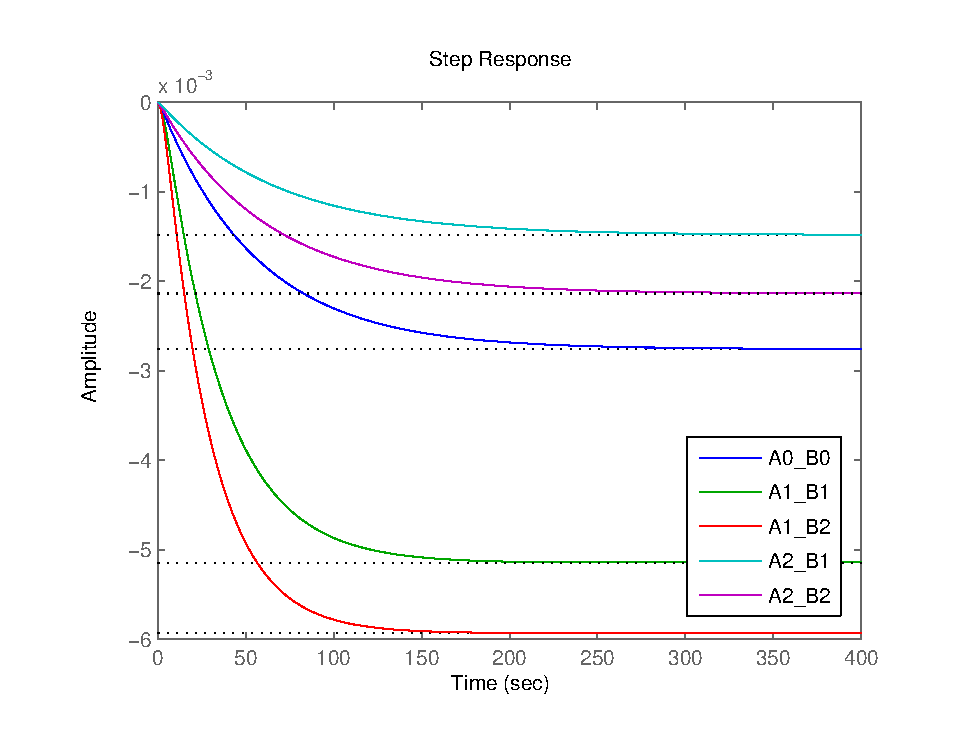
\includegraphics[width=1\columnwidth]{figures/h2_polytopic.eps}
	\caption{Resposta do sistema (\ref{eq:sis_mf_incerteza}) com o ganho K encontrado 
		pelo crit�rio de $H_2$}
	\label{fig:h2_polytopic}
\end{figure}

%===============================================================================
\subsection{Incertezas limitadas em norma}
\label{sec:normh2_norm_limit}

Para o caso de incertezas com norma limitada temos (\ref{eq:normh2_norm_limit}).


\begin{equation}
\begin{matrix}
\gamma _2^2 > Tr(B_{\omega}'W^{-1}B_{\omega})
\\ 
\\
\begin{bmatrix}
Y & (E_AW-E_BR)' & (GW-HR)'\\ 
(E_AW-E_BR) & I & 0\\ 
 (GW-HR) & 0 & I
\end{bmatrix} \geq 0
\\ 
\\ 
Y=-WA_0'+R'B_0'-A_0W +B_0R -DD'
\end{matrix}
\label{eq:normh2_norm_limit}
\end{equation}

Com a realimenta��o $K=RW^{-1}$.
%===============================================================================
\subsubsection{Simula��o}

A resolu��o do sistema de LMIs (\ref{eq:normh2_norm_limit}) gerou os seguintes resultados:

\begin{equation}
\begin{matrix}
W=\begin{bmatrix}
0.4644 &  -0.0305\\
-0.0305 &   0.7975
\end{bmatrix}\\ \\ 
R=1.10^3\begin{bmatrix}
0.0009 &  -8.6987
\end{bmatrix}
\\ \\
K=1.10^4\begin{bmatrix}
-0.0716 &  -1.0935
\end{bmatrix}
\\ \\
M =  0.0170
\\
\lambda_1=-0.0326\\
\lambda_2=-1.7666
\end{matrix}
\nonumber
\end{equation}

A simula��o do sistema em malha fechada com o ganho $K$ encontrado obtem a resposta
apresentada na Figura (\ref{fig:h2_norm_bounded}). Os valores de $\lambda_1$ e $\lambda_2$ 
s�o os autovalores do sistema em malha fechada.

\begin{figure}[htbp]
	\center
	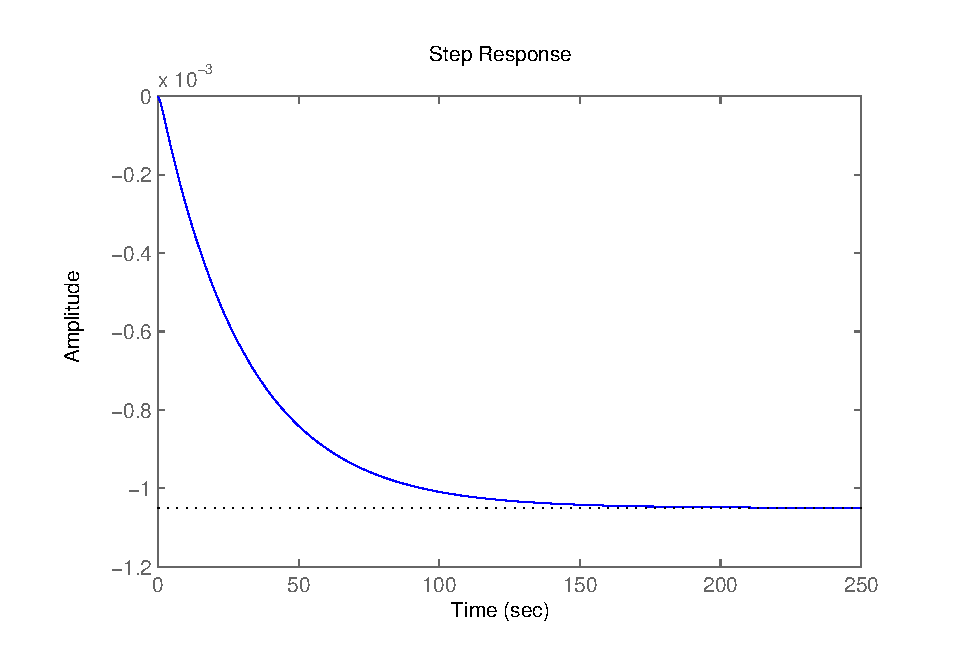
\includegraphics[width=1\columnwidth]{figures/h2_norm_bounded.eps}
	\caption{Resposta do sistema (\ref{eq:sis_mf_incerteza}) com o ganho K encontrado 
		pelo crit�rio de $H_2$}
	\label{fig:h2_norm_bounded}
\end{figure}

%===============================================================================
\section{Norma $H_{\infty}$}
\label{sec:normHinf}

Para o sistema apresentado em (\ref{eq:robust_sis_incert}) a norma $L_2$ deste sistema
� definido como em (\ref{eq:normhinf_l2}).

\begin{equation}
\underset{\left \| \omega(t) \right \|_2 \neq 0}{sup}=\frac{\left \| z(t) \right \|_2}{\left \| \omega(t) \right \|_2}
\label{eq:normhinf_l2}
\end{equation}

Onde a norma $L_2$ de um sinal $\omega(t)$ � definida como abaixo:

\begin{equation}
\left \| \omega(t) \right \|_2 \equiv \sqrt{\int_{0}^{\infty}\omega(t)'w(t) dt}
\nonumber
\end{equation}

Suponha que exista uma fun��o quadr�tica positiva $V(x)=x'Px$ com $P=P'>0$ e um escalar positivo
$\gamma_{\infty}$ tal que:


\begin{equation}
\dot{V}z(t)'z(t)-\gamma_{\infty}^{\omega}\omega(t)'\omega(t)\leq 0
\nonumber
\end{equation}
%===============================================================================
\subsection{Sistemas Lineares sem incertezas}
\label{sec:hinf_sis_lin_sem_incertezas}

Considerando o sistema apresentado em (\ref{eq:robust_sis_incert}) em malha fechada, com 
condic�o inicial nula ($x(0)\equiv 0$) e com $ \Delta (t) \equiv 0$, obtem-se desta forma
o sistema apresentado em (\ref{eq:sis_mf_incerteza}).

\begin{equation}
\left\{\begin{matrix}
\dot{x}(t)=(A_0-B_0K)x(t)+B_{\omega}\omega(t)\\ 
z(t)=(G-HK)x(t)
\end{matrix}\right.
\label{eq:sis_mf_incerteza}
\end{equation}

A LMI que deve ser satisfeita para que a confic�o de $H_{\infty}$ seja obtida � apresentada
em (\ref{eq:hinf_sem_incerteza}).

\begin{equation}
\begin{bmatrix}
-WA_0'+R'B_0'-A_0W-B_0R-B_{\omega}B_{\omega}' & -(GW-HR)'\\ 
 -(GW-HR) & \gamma_{\infty}^2 I  
\end{bmatrix}\geq 0
\label{eq:hinf_sem_incerteza}
\end{equation}

Assim pode-se garantir o limite superior min�mo para o ganho $L_2$ do sistema 
(\ref{eq:sis_mf_incerteza}).

Para o caso de sistemas lineares invariantes no tempo a otimizac�o d� exatamente o valor do
ganho $L_2$ que � igual a norma $H_{\infty}$. 

\begin{equation}
T(s)=(G-HK)(sI-(A_0-B_0K))^{-1}B_{\omega}
\nonumber
\end{equation}

Que � equivalente a:

\begin{equation}
\left \| T(s) \right \|_{\infty} \equiv \underset{\omega \in \Re}{max}\sqrt{\lambda (T'(j\omega)T(j\omega))}
\nonumber
\end{equation}

%===============================================================================
\subsection{Incertezas do tipo polit�pico}
\label{sec:hinf_sis_politopico}

No caso de incertezas do tipo polit�picas o limite superior minimo para o ganho $L_2$ pode ser
definido pela equac�o (\ref{eq:hinf_sis_politopico}).

\begin{equation}
\begin{matrix}
\begin{bmatrix}
Y & -(GW-HR)'\\ 
-(GW-HR) & \gamma_{\infty}^2
\end{bmatrix}\geq 0
\\ 
\\ 
Y=-WA_i'+R'B_j'-A_iW+B_jR-B_{\omega}B_{\omega}'
\\ \\
W>0
\end{matrix}
\label{eq:hinf_sis_politopico}
\end{equation}


%===============================================================================
\subsection{Incertezas limitadas em norma}
\label{sec:hinf_sis_norm_limit}

Considerando o sistema descrito em (\ref{eq:robust_sis_incert}) com $\left \| \Delta(t) \right \|\leq 1$.
A condic�o descrita em (\ref{eq:hinf_sem_incerteza}) � equivalente a (\ref{eq:hinf_sis_norm_lim}).

\begin{equation}
\begin{matrix}
\begin{bmatrix}
Y &(E_AW-E_BR)' & -(GW-HR)'\\ 
(E_AW-E_BR) & I & 0\\
-(GW-HR) & 0& \gamma_{\infty}^2
\end{bmatrix}\geq 0
\\ 
\\ 
Y=-WA_0'+R'B_0'-A_0W+B_0R-B_{\omega}B_{\omega}'
\\ \\
W>0
\end{matrix}
\label{eq:hinf_sis_norm_lim}
\end{equation}

Satisfazendo a equac�o (\ref{eq:hinf_sis_norm_lim}) obtem-se o limite superior minimo para o
ganho $L_2$ e se o sistema for linear e invariante no tempo este valor ser� o mesmo da norma 
$H_{\infty}$ da func�o de transferencia entre $\omega$ e $z$.


%===============================================================================

%===============================================================================
\section{Sistema Nominal - Centro das incertezas}
\label{sec:nominal}

%===============================================================================

\section{Conclus�es}
\label{sec:concl}

Foi apresentado neste trabalho uma breve descri��o do funcionamento do
Filtro de Kalman, suas in�meras aplica��es nas mais diversas atividades
e ramos da engenharia moderna. Apresentou-se o diferencial da utilizac�o 
do filtro devido a sua robustez para implementa��o no que diz respeito ao
mundo digital e sua robustez quando existe ruido ou incerteza na planta em
quest�o.

Apresentou-se tamb�m o problema de LQR para tempo discreto, sua modelagem
e a realiza��o do filtro de kalman pelo principio da separa��o, onde a
modelagem do filtro pode ser entendida/resolvida pela resolu��o de um problema
de LQR e outro de LQG.

Apresentou-se tamb�m dois tipos principais para a realiza��o do filtro de kalman:
realiza��o por estima��o (\ref{fig:kalman_bucy_filter}) e a realiza��o em 
cascata (\ref{fig:cascade_realization}).

Com estes pontos apresentados aqui e com a grande aplicabilidade dos filtros
de kalman em problemas comuns da engenharia, observamos que este aparato
tem grande import�ncia e suas aplica��es (\ref{sec:applications}) n�o se 
restringem �s apresentadas neste trabalho.



\bibliographystyle{IEEEtran}
\bibliography{biblio}

\end{document}
